%=====================================================================
\subsection{The MUSCL-Hancock Method} \label{chap:MUSCL-hancock}
%=====================================================================











%======================================================
\subsubsection{Method}
%======================================================

The MUSCL-Hackock method is a method of the class of \textbf{M}onotone \textbf{U}pwind \textbf{S}chemes for \textbf{C}onservation \textbf{L}aws, which try to achieve higher order accuracy by describing the states $\U_i$ of each cell $i$ not by a constant state, but by some higher order interpolation.
The MUSCL-Hanckock scheme in particular assumes a piecewise linear state reconstruction, see fig. \ref{fig:piecewise-linear} for an example.


\begin{figure}[H]
	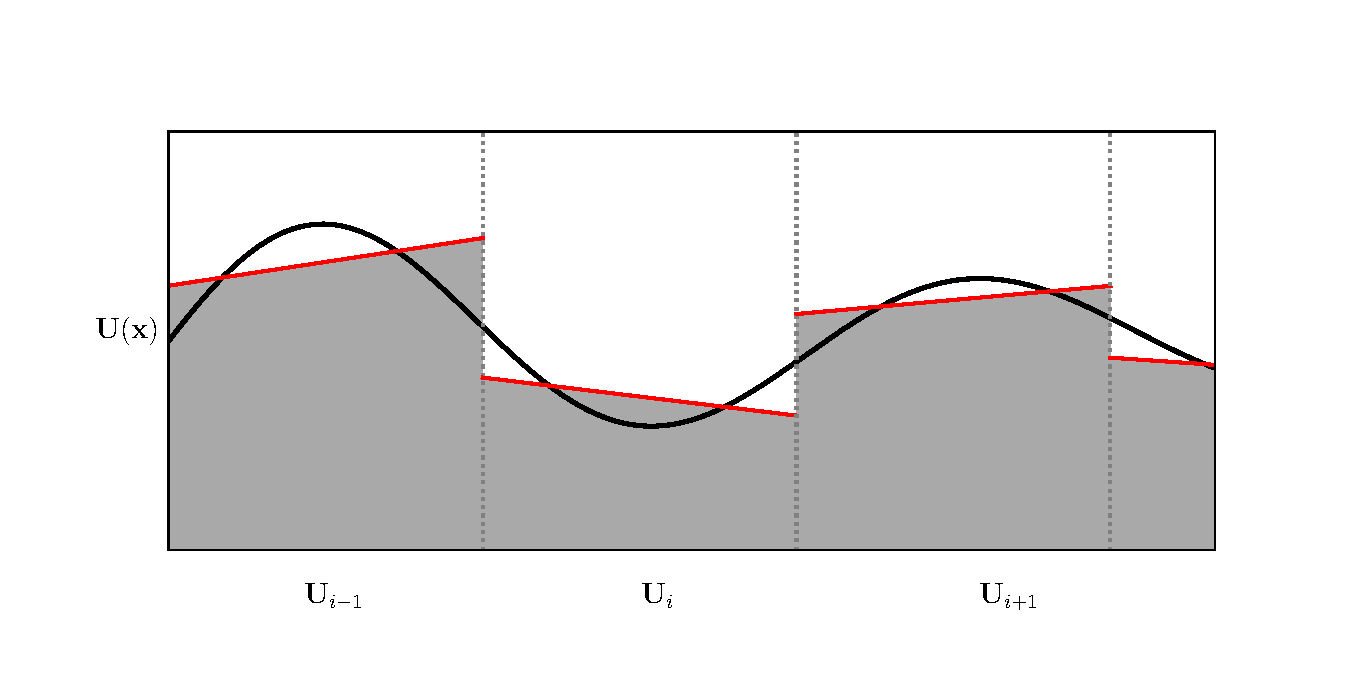
\includegraphics[width=\textwidth]{./figures/piecewise_linear.pdf}%
	\caption{	
		A piecewise linear representation of continuous data among cells.
		\label{fig:piecewise-linear}
		}
\end{figure}


It solves the hyperbolic conservation law of the form

\begin{equation*}
	\DELDT{\U} + \DELDX{\F(\U))} = 0
\end{equation*}

just like all other schemes so far using the explicit conservative formula

\begin{equation}
	\U_i^{n+1} = \U_i^n + \frac{\Delta t}{\Delta x} \left( \F_{i-\half} - \F_{i + \half} \right)
\end{equation}

where $\U_i$ is the volume average of a state in a cell, which is however not constant throughout the cell, but is described by

\begin{equation}
	\U_{i}(x) = \U_i^n + \frac{x - x_i}{\Delta x} \mathbf{s}_i; \quad x \in [0, \Delta x]
\end{equation}


$\mathbf{s}_i$ is a suitably chosen slope vector of $\U_i(x)$ in cell $i$.
A general slope can be written as

\begin{equation}
 	\mathbf{s}_i = \frac{1}{2} (1 + \omega) (\U_i - \U_{i-1}) + \frac{1}{2} (1 - \omega) (\U_{i+1} - \U_i)
\end{equation}

with $\omega \in [-1, 1]$.
For $\omega = 0$, we retrieve the centered scheme.
$\omega = 1$ gives us the upwind slope, $\omega = -1$ gives us the downwind slope.
In the code, $\omega$ can be set as a compile time macro \texttt{OMEGA} in \texttt{defines.h}.


However, having non-constant states creates a problem for Riemann solvers.
We now need to solve the so called \emph{Generalised Riemann Problem} with

\begin{align}
	\DELDT{\U} + \DELDX{\F(\U))} &= 0 \\
	\U(x, 0) &= 
	\begin{cases}
		\U_i(x), & \quad x < 0 \\
		\U_{i+1}(x), & \quad x > 0 \\
	\end{cases}
\end{align}

As the left and right states change with $x$, the characteristics are no longer straight lines, which makes things tricky.
So instead of dealing with that analytically, the MUSCL-Hancock method tries to compute some sort of ``intermediate state'' such that in the end, we get an approximate flux that is good enough for our purposes.

In each cell, the extreme values are located at the cell boundaries.
They are referred to as boundary extrapolated values, and are given by

\begin{equation}
	\U_i^L = \U_i^n - \frac{1}{2} \mathbf{s}_i; \quad 	\U_i^R = \U_i^n + \frac{1}{2} \mathbf{s}_i; 
\end{equation}


To obtain a second order intercell flux, we first try and find intermediate extrapolated boundary values by applying the same conservative explicit formula on every cell separately over half the timestep.
We denote the intermediate boundary extrapolated values as $\overline{\U}_i^L$ and $\overline{\U}_i^R$, and obtain them by computing

\begin{align}
	\overline{\U}_i^L &= \U_i^L + \frac{1}{2} \frac{\Delta t}{\Delta x} \left( \F(\U_i^L) - \F(\U_i^R) \right)\\
	\overline{\U}_i^R &= \U_i^R + \frac{1}{2} \frac{\Delta t}{\Delta x} \left( \F(\U_i^L) - \F(\U_i^R) \right)
\end{align}

Note that this update depends only on the values inside a cell, and can be computed for every cell individually.

Finally, with the evolved boundary extrapolated values, we can compute the fluxes $\F_{i + \half} = \F(\U_{i+\half}(x = 0))$ by solving the Riemann problem at every cell interface and using the initial values

\begin{align}
	\U_L &= \overline{\U}_i^R\\
	\U_R &= \overline{\U}_{i+1}^L 
\end{align}

and by sampling the solution at $x = 0$.


Note that we only use the intermediate evolved state to estimate the evolved boundary extrapolated values, which in their turn are used to obtain left and right initial values for the Riemann problem.
We don't use the evolved state when finally evolving the state!

So in short, what we need to do is

\begin{itemize}
	\item 	Compute slope $\mathbf{s}_i$ for each cell
	\item 	find evolved boundary extrapolated values using 
			\begin{align*}
				\overline{\U}_i^L &= \U_i^L + \frac{1}{2} \frac{\Delta t}{\Delta x} \left( \F(\U_i^L) - \F(\U_i^R) \right)\\
				\overline{\U}_i^R &= \U_i^R + \frac{1}{2} \frac{\Delta t}{\Delta x} \left( \F(\U_i^L) - \F(\U_i^R) \right)
			\end{align*}
	\item 	find fluxes $\F_{i + \half}$ as $\F(\U_{i+\half})$ with $\U_{i+\half}$ being the solution to the Riemann problem 
			\begin{align}
				\U_L &= \overline{\U}_i^R\\
				\U_R &= \overline{\U}_{i+1}^L 
			\end{align}
			at $ x = 0$

	\item 	update the state using 
			\begin{equation}
				\U_i^{n+1} = \U_i^n + \frac{\Delta t}{\Delta x} \left( \F_{i-\half} - \F_{i + \half} \right)
			\end{equation}
\end{itemize}




A TVD version is obtained by using slope limiters, i.e. replacing the slope $\mathbf{s}_i$ by a limited slope $\overline{\mathbf{s}}_i$ with

\begin{align*}
	\overline{\mathbf{s}}_i &= \xi(r) \mathbf{s}_i \\
	r &= \frac{\U_i - \U_{i-1}}{\U_{i+1} - \U_{i}} \quad\quad \text{for each component of }\U
\end{align*} 

some possible and implemented slope limiters $\xi(r)$ are given in section \ref{chap:implemented_limiters}.
















%======================================================
\subsubsection{Implementation Details}
%======================================================




The cells are stored just like in the Godunov method.
Additionally, we need to store the evolved extrapolated boundary states $\overline{\U}_i^L$ and $\overline{\U}_i^R$ for each cell.


The flux at $x_{i+\half, j}$ and $y_{i, j+\half}$ are stored in \texttt{cflux}of cell \verb|grid[i, j]|.
Because we're doing dimensional splitting, it suffices to have only one storage place, as they will be used in successive order.
See section \ref{chap:dimensional-splitting} for details.

We can afford to store $x_{i+\half}$ at cell $i$ because we have at least 2 extra virtual boundary cell which is used to apply boundary conditions, so the flux at $x_{-\half}$ will be stored in \verb|grid[BC-1]|, where \texttt{BC} is the number of boundary cells used, defined in \texttt{defines.h}.
 



The related functions are written in \texttt{/program/src/solver/muscl.c} and \texttt{/program/src/solver/muscl.h}.
The hydro related functions are called in the main loop in \texttt{/program/src/main.c} when \verb|solver_step(...)| is called.

The \verb|solver_step(...)| function does the following for the 1D case:
\begin{itemize}
	\item 	Reset the stored fluxes from the previous timestep to zero
	\item 	Compute the primitive states for all cells from the updated conserved states
	\item 	Impose boundary conditions (section \ref{chap:boundary-conditions})
	\item 	Find the maximal timestep that you can do by applying the CFL condition \ref{eq:godunov-cfl}.
	\item 	Compute fluxes:
	\begin{itemize}
		\item 	For every cell, find the (limited) slope $\mathbf{s}_i$ and then compute the evolved extrapolated boundary states $\overline{\U}_i^L$ and $\overline{\U}_i^R$ for each cell.
				We need to solve the Riemann problem with $\U_L = \overline{\U}_i^R$, $\U_R = \overline{\U}_{i+1}^L$ later, so those values need to be present for the neighbouring cells before we can compute the Riemann problem.
				This is done by first computing the evolved boundary extrapolated states in a single loop over all cells, and then the rest of the solution is done in a second loop over all cells.
		\item 	For every cell pair $(i, i+1)$, solve the Riemann problem (see section \ref{chap:riemann}) to find the flux $\F_{i+\half}$ with $\U_L = \overline{\U}_i^R$, $\U_R = \overline{\U}_{i+1}^L$.
		\item 	Store the flux $\F_{i+\half}$ in the \texttt{struct cstate cflux} struct of the cell $i$.
				\texttt{struct cstate} is a struct that contains the conserved states, i.e. density $\rho$, momentum $\rho u_x$, $\rho u_y$, and energy $E$.
	\end{itemize}
	\item 	Update the states: Effectively compute $\U^{n+1}$ at this point using $\U_i^n$, the flux $\F_{i+\half}$ stored in every cell $i$, and the flux $\F_{i-\half}$ stored in every cell $i-1$.
\end{itemize}
